\documentclass[11pt]{article}
\usepackage[utf8]{inputenc}
\usepackage[french]{babel}
\usepackage[margin=1in]{geometry}
\usepackage{amsfonts, amsmath, amssymb}
\usepackage[none]{hyphenat}
\usepackage{fancyhdr}
\usepackage{graphicx}
\usepackage{float}
\usepackage[nottoc, notlot, notlof]{tocbibind}
\usepackage{array,multirow,makecell}
\setcellgapes{1pt}
\makegapedcells
\usepackage[table]{xcolor}
\usepackage{import}
\usepackage{tikz}
\usepackage{hyperref}
\usepackage{enumitem}
\usepackage{chemist}
\usepackage{arydshln}

\pagestyle{fancy}
\fancyhead{}
\fancyfoot{}
\fancyhead[L]{Gymnase Auguste Piccard}
\fancyhead[R]{2021-2022}
\fancyfoot[R]{\thepage}
\renewcommand{\footrulewidth}{0pt}
\renewcommand{\headrulewidth}{0pt}

\def \hfillx {\hspace*{ -\textwidth} \hfill}

\setlength\arrayrulewidth{1pt}

\begin{document}
\huge
\begin{minipage}{.5\textwidth}%
\begin{flushleft}
\underline{Laboratoire n° 3} \\
\normalsize Romain Blondel, Nicola Badic
\end{flushleft}
\end{minipage}
\begin{minipage}{.5\textwidth}%
\begin{flushright}
\huge
Note \normalsize\textit{(compte double)} \huge :\hrulefill
\end{flushright}
\end{minipage}
\begin{center}
\textbf{Distillation d’un vin rouge} \\
\scriptsize Adapté du TP « Distillation d’un vin rouge » de M. Julien Falcy, enseignant à Auguste Piccard. Merci à lui ! 
\end{center}
\normalsize
\section*{Buts}
\begin{itemize}
\item[•]Comprendre les principes de la distillation
\item[•]Distiller 65 mL de vin rouge 
\item[•]Calculer la teneur en alcool du distillat puis la teneur en alcool du vin rouge.
\end{itemize}
\section*{Introduction théorique}
\subsection*{1. Le vin rouge}
Le  vin  rouge  est  un  mélange  homogène  complexe  d’environ  500  composés.  La  variation  de  leurs concentrations  offre  à  chaque  vin  des  propriétés  organoleptiques  uniques  (robe,  bouquet  et  saveur). Parmi ses composés, on compte notamment :\\
\begin{minipage}{.2\textwidth}%
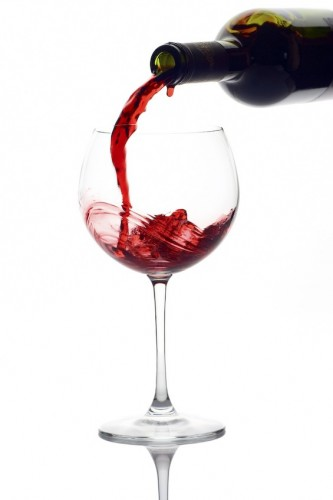
\includegraphics[scale=0.3]{vin1.jpg}
\end{minipage}
\begin{minipage}{.8\textwidth}%
\begin{itemize}
\item[•]Eau\footnotemark[1], qui est le solvant du mélange ; 
\item[•]Ethanol\footnotemark[2] (\chemform{C_2H_5OH}), qui est le soluté présent en plus grande quantité ; 
\item[•]Glycérol ;
\item[•]Acides organiques, dont l’acide tartrique, malique, lactique et succinique ;
\item[•]Sucres ;
\item[•]Minéraux ;
\item[•]Arômes, dont les tanins ;
\item[•]Colorants ;
\item[•]Vitamines, principalement la famille des B et C$_2$.
\end{itemize}
\end{minipage}\\ 
Le  moût  de  raisin  est  transformé  en  vin  rouge  au  cours  d'un  procédé  appelé  \textbf{vinification},  durant laquelle  toute  une  suite  de  transformations  physiques,  biologiques  et chimiques  ont  lieu.  Parmi  les transformations biologiques, deux \textbf{fermentations}  successives ont lieu à l'aide de microorganismes.
\begin{enumerate}[label=\alph*)]
\item La \textbf{fermentation alcoolique} transforme le glucose (\chemform{C_6H_12O_6}) du moût en éthanol et \chemform{CO_2} :
\begin{chemmath}
\centering
C_6H_12O_6 \xrightarrow{Levure} 2 C_2H_5OH + 2 CO_2
\end{chemmath}
\item La \textbf{fermentation malolactique} transforme l'acide malique (\chemform{C_4H_6O_3}) en acide lactique (\chemform{C_3H_6O_3}) et \chemform{CO_2} :
\begin{chemmath}
\centering
C_4H_6O_5 \xrightarrow{Oenococcus \: oeni} C_3H_6O_3 + CO_2
\end{chemmath}
\end{enumerate}

\subsection*{2. La teneur alcoolique}
La  teneur  en  alcool  d'une  boisson  alcoolisée  se  mesure  en  \textbf{volumes \%} \: $[vol \: \%]$.  Elle représente  le volume d’éthanol  pur contenu  dans  la boisson.  Ainsi  un vin  rouge  dont l'étiquette  indique  $12 \: vol \: \%$ contient $12 \: mL$ d’éthanol pur sur $100 \: mL$ de vin.
\footnotetext[1]{T\begin{tiny}
ébullition
\end{tiny}(\chemform{H_2O}) = 100 °C}
\footnotetext[2]{T\begin{tiny}
ébullition
\end{tiny}(Ethanol) = 78.4 °C}
\clearpage
\subsection*{3. La distillation fractionnée}
La  distillation   est  une  technique   de  séparation   de  deux  liquides   miscibles   en  fonction  de  leur température  d'ébullition.  Dans  un  mélange  eau-éthanol  porté  à  80  °C,  deux  phénomènes  physiques distincts sont observés :\\
\begin{minipage}{.6\textwidth}%
\begin{itemize}
\item[•] Évaporation de l'eau
\item[•] Ébullition de l'alcool
\end{itemize}
La  colonne  Vigreux  permet  une  bonne  séparation  des constituants  du  mélange.  En  effet,  
lorsque  les  vapeurs montent    dans   la   colonne,    elles   refroidissent    et   se 
condensent  sur les aiguilles  de la colonne.  Ce  liquide  est ensuite   à   nouveau   chauffé   
progressivement   par   les vapeurs  qui continuent  de monter, jusqu'à être vaporisé à nouveau.\\

A    cause    de    toutes    ces    vaporisations-condensations successives,  l'eau  retombe  et  
les  vapeurs  montantes  sont de plus en plus chargées en éthanol.
\end{minipage}
\begin{minipage}{.4\textwidth}%
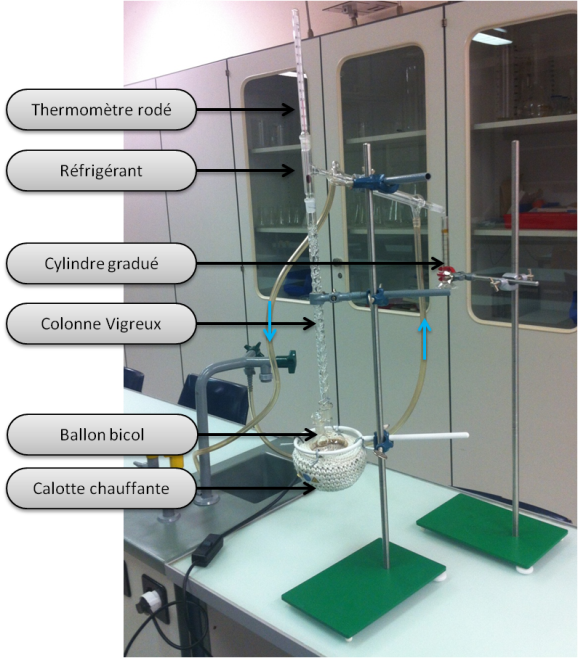
\includegraphics[scale=0.25]{vin2.png}
\end{minipage}\\

\section*{Montage}
\begin{enumerate}
\item Avant tout ; évitez de forcer sur les rodages.
\item Le ballon bicol est placé dans la calotte chauffante.
\item La  colonne  Vigreux  est  attachée  verticalement  sur  le  ballon  à  l'aide  d'un  clip  
de  sécurité  et  le second col est fermé avec le bouchon rodé.
\item La calotte est attachée au statif à l'aide d'un cercle et la colonne Vigreux à l'aide d'une 
pince.
\item Un réfrigérant à eau est placé au-dessus de la colonne Vigreux et un thermomètre rodé est 
placé à son sommet.
\item Le cylindre gradué est maintenu à la sortie du réfrigérant à l'aide d'une pince et d'un 
statif.
\end{enumerate}

\section*{Méthode}
\begin{enumerate}
\item Peser les deux cylindres gradués de $10 \: mL$ (noter les résultats précis sur la page suivante).
\item Monter l'appareil à distiller selon les instructions données ci-dessus.
\item Introduire 2-3 pierres à distiller et $65 \: mL$ de vin rouge dans le ballon de $250 \: mL$.
\item Faire contrôler le montage par l'enseignant.
\item Allumer l'eau du réfrigérant puis enclencher la calotte chauffante au maximum.
\item Dès le début de l'ébullition,  un front de vapeur d’éthanol monte dans la colonne Vigreux. 
Afin de
garantir  une bonne séparation  eau-éthanol,  l'ascension  ne doit pas se faire en moins de $2 \: min$. 
Il faut alors jouer avec la puissance de la calotte ; en l’allumant/arrêtant, voir en la 
descendant.
\item Dès la première  goutte de distillat  obtenue  dans le  le cylindre gradué,  la température  
de vapeur est notée tous les $0.5 \: mL$ de distillat écoulés.
\item Lorsque  la température  dépasse  82 °C,  le distillat  est récolté  dans le 2$^e$ cylindre  
gradué.  Le but est d'obtenir 6 à 7 ml de distillat dans ce second cylindre gradué.
\end{enumerate}
\clearpage
\section*{Résultats \& Compte-rendu (partie 1) : Relevé de températures}
Nom du vin = Sualdeia \\
V\begin{tiny}vin prélevé\end{tiny} = $65 \: mL$\\
Teneur alcoolique\begin{tiny}vin\end{tiny} (indiqué sur l'étiquette) = 13 $vol. \%$ d'éthanol
\begin{table}[H]
\centering
\arrayrulecolor{orange}
\begin{tabular}{|l|l|}
\hline
\rowcolor{orange} Distillat 1 & Distillat 2 \\
\hline
m\begin{tiny}cylindre 1 (vide)\end{tiny} = $32.077 \: g$ & m\begin{tiny}cylindre 2 (vide)\end{tiny} = $19.210 \: g$ \\
m\begin{tiny}cylindre 1 (plein)\end{tiny} = $37.047 \: g$ & m\begin{tiny}cylindre 2 (plein)\end{tiny} = $24.675 \: g$ \\
m\begin{tiny}distillat (1)\end{tiny} = $4.970 \: g$ & m\begin{tiny}distillat (2)\end{tiny} = $5.465 \: g$ \\
V\begin{tiny}distillat (1)\end{tiny} = $6 \: mL$ & V\begin{tiny}distillat (2)\end{tiny} = $6 \: mL$ \\
\hline
\end{tabular}
\end{table}

\begin{table}[H]
\arrayrulecolor{black}
\caption{Température des vapeurs en tête de colonne en fonction du volume de distillat \\ \textit{\textbf{À relever tous les 0.5 mL, jusqu'à un total d'environ 12 mL de distillat}}}
\begin{minipage}{0.33\textwidth}
\begin{tabular}{l:l}
\hline
V\begin{tiny}distillat\end{tiny} [mL] & T\begin{tiny}vapeur\end{tiny} [°C]\\
\hline
\rowcolor{lightgray}0.0 & 74.0 \\  
1.0 & 75.0 \\  
\rowcolor{lightgray}1.5 & 75.5 \\  
2.0 & 75.5 \\  
\rowcolor{lightgray}2.5 & 76.0 \\  
3.0 & 76.0 \\  
\rowcolor{lightgray}3.5 & 76.5 \\  
4.0 & 76.5 \\  
\rowcolor{lightgray}4.5 & 76.5 \\ 
\hline
\end{tabular}
\end{minipage}
\begin{minipage}{0.33\textwidth}
\begin{tabular}{l:l}
\hline
V\begin{tiny}distillat\end{tiny} [mL] & T\begin{tiny}vapeur\end{tiny} [°C]\\
\hline
\rowcolor{lightgray}5.0 & 76.5 \\  
5.5 & 77.5 \\  
\rowcolor{lightgray}6.0 & 80.0 \\ \hline  
6.0 & 82.0 \\  
\rowcolor{lightgray}7.0 & 90.0 \\  
7.5 & 92.0 \\  
\rowcolor{lightgray}8.0 & 93.0 \\  
8.5 & 93.5 \\  
\rowcolor{lightgray}9.0 & 94.0 \\ 
\hline
\end{tabular}
\end{minipage}
\begin{minipage}{0.33\textwidth}
\begin{tabular}{l:l}
\hline
V\begin{tiny}distillat\end{tiny} [mL] & T\begin{tiny}vapeur\end{tiny} [°C]\\
\hline
\rowcolor{lightgray}9.5 & 95.0 \\  
10.0 & 96.0 \\  
\rowcolor{lightgray}10.5 & 96.0 \\  
11.0 & 97.0 \\  
\rowcolor{lightgray}11.5 & 97.0 \\  
12.0 & 97.0 \\
\rowcolor{lightgray} & \\
 & \\ 
\rowcolor{lightgray} & \\
\hline
\end{tabular}
\end{minipage}
\end{table}
\textit{Note : la ligne et la double apparition de $V = 6 \: [mL]$ correspondent au changement de cylindre.}

\section*{Discussion des résultats (partie I)}
\begin{enumerate}
\item Représentez  graphiquement  (main  ou  excel),  à  l'aide  des  valeurs  ci-dessus,  l'évolution  de  la température de vapeur en tête de la colonne en fonction du volume de distillat ! Le graphique doit porter un titre, les axes également, ainsi que des unités, et n'oubliez pas vos légendes.
\item Discutez \underline{de manière détaillée} l'évolution de cette courbe.
\end{enumerate}
\subsection*{1. Graphe}
\begin{figure}[H]
\caption{Variation de la température en fonction du volume du distillat}
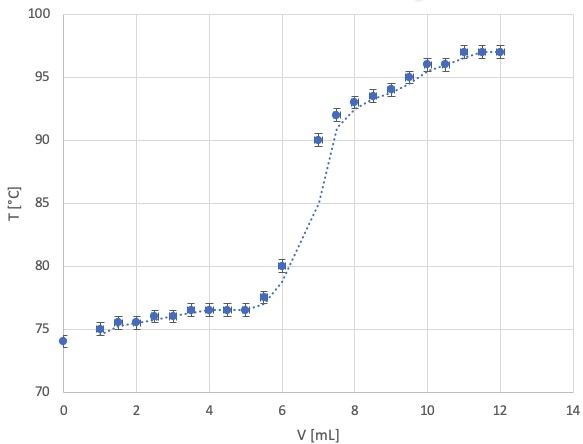
\includegraphics[scale=1]{SAVE_20211208_165531.jpg}
\end{figure}
\textit{Note : Le points bleus sont les mesures effectuée (cf. Table 1) incluant une incertitude tel qu'énoncé plus tard. Le traitillé bleu est une courbe de tendance afin de faciliter la lisibilité du graphe.}

\subsection*{2. Discussion}
On peut prendre ce graphique en trois parties : la première de 0 à 5.5 [mL] où la température n'augmente que peu, la seconde entre 6 et 8 [mL], où la température va fortement augmenter et un troisième partie dès 8 [mL] avec un variation de température semblable au début.\\ 
L'éthanol et l'eau étant les composants majoritaires du vin, et que l'éthanol ayant une température d'ébullition moindre que l'eau, on peut assez sûrement dire que la première partie du graphe correspond à l'évaporation de celui-ci. De plus, la fourchette de température est proche de celle de la vaporisation de l'éthanol (entre 74 et 80 [°C] pour 78.4 [°C]). \\
La majorité de l'éthanol étant évaporé, la seconde partie correspond à l'augmentation de température avant l'évaporation de l'eau. Cela coïncide avec le changement de cylindre. \\
La dernière partie correspond donc à l'évaporation de l'eau avec la l'éthanol qui n'a pas pu s'évaporer avant (comme on le constate dans la partie suivante).
\clearpage

\section*{Résultats \& Compte-rendu (partie 2) : Analyse des deux distillats}
\subsection*{1. Distillat 1}
\begin{itemize}
\item[•] $\rho_{distillat \: 1} \: \left( en \: \frac{g}{mL} \: puis \: en \: \frac{g}{L} \right) = \frac{4.97}{6}\left[\frac{g}{mL}\right] = 0.828\overline{3} \left[\frac{g}{mL}\right] = 828.\overline{3} \left[\frac{g}{L}\right]$
\item[•] Teneur alcoolique\begin{tiny}(distillat 1)\end{tiny} = (à trouver sur le graphique) = $86 [vol. \%]$
\item[•] V\begin{tiny}éthanol (distillat 1)\end{tiny} $= 86 \% \cdot 6 = 5.16 [mL]$ 
\end{itemize}

\subsection*{2. Distillat 2}
\begin{itemize}
\item[•] $\rho_{distillat \: 1} \: \left( en \: \frac{g}{mL} \: puis \: en \: \frac{g}{L} \right) = \frac{5.465}{6}\left[\frac{g}{mL}\right] = 0.9108\overline{3} \left[\frac{g}{mL}\right] = 910.8\overline{3} \left[\frac{g}{L}\right]$
\item[•] Teneur alcoolique\begin{tiny}(distillat 2)\end{tiny} = (à trouver sur le graphique) = $51 [vol. \%]$
\item[•] V\begin{tiny}éthanol (distillat 2)\end{tiny} $= 51 \% \cdot 6 = 3.06 [mL]$ 
\end{itemize}

\subsection*{3. Total \textit{(distillat 1 + distillat 2)}}
\begin{itemize}
\item[•] V\begin{tiny}éthanol, total\end{tiny} $= 5.16 + 3.06 = 8.22 [mL]$ 
\item[•] Teneur alcoolique\begin{tiny}vin\end{tiny} $= \frac{8.22}{65} \approx 12.65 [vol. \%]$ 
\end{itemize}
\section*{Discussion des résultats (partie II)}
\begin{enumerate}
\item Calculez  les  \textbf{erreurs  absolue} et \textbf{relative}  de  votre  expérience  (voir  laboratoire  n°  1)  afin  de comparer les valeurs de la teneur alcoolique  théorique (sur la bouteille) et pratique.
\item Discutez des causes d'erreurs possibles de manière précise et détaillée (au moins 4).
\end{enumerate}
\subsection*{1. L'erreur}
\begin{itemize}
\item[•]Erreur absolue : Valeur théorique - Valeur obtenue (en valeur absolue) $\Rightarrow$ $\lvert 13 - 12.65 \rvert = \lvert 0.35 \rvert = 0.35$, soit une erreur absolue de 0.35 $[vol \%]$.
\item[•] Erreur relative : Erreur absolue / Valeur théorique $\Rightarrow$ $\frac{0.35}{13} \approx 2.69 \%$.
\end{itemize}

\subsection*{2. Discussion}
L'erreur peut venir de nombreux facteurs. Celui le plus évident est l'observateur et l'instrument de mesure (précision de la mesure par l'un comme l'autre). \\
Ensuite, le déroulement de l'expérience met en jeu certains facteurs incontrôlable, comme une infime partie du liquide pouvant rester coincé dans la colonne, la "vitesse" d'évaporation de différents composants (soit la durée de l'expérience) peut faire varier légèrement les résultats (la proportion d'éthanol dans les différents distillats). \\
De plus, on considère plusieurs faits comme vrai afin de faciliter la mesure, comme l'évaporation totale de l'éthanol à la fin de l'expérience (qui n'est probablement pas vrai) ainsi que le graphique utilisé pour trouver la proportion d'éthanol peut être que partiellement exacte et relativement imprécis dans le cadre de ces mesures.\\
 Finalement, la valeur théorique donnée par le producteur de vin peut être inexacte (légalement de $\pm 0.5 \: [vol \%]$).

\paragraph*{Note : l'incertitude des mesures -}
Si l'on considère selon les conventions que l'incertitude d'une mesure et la moitié de "l'unité" de l'appareil de mesure, celle de la température et $\pm 0.5$ [°C], du volume de liquide $\pm 0.1$ [mL] et pour la masse $\pm 0.0005$ [g]. Donc l'incertitude de la masse de distillat est de $\pm 0.001$ [g] ($= 0.0005 + 0.0005$), puis sur la masse volumique $\frac{\Delta \rho _{distillat 1}}{\rho _{distillat 1}}  = \frac{0.001}{4.97} + \frac{0.1}{6} \approx 1.69 \%$ et $\frac{\Delta \rho _{distillat 2}}{\rho _{distillat 2}}  = \frac{0.001}{5.465} + \frac{0.1}{6} \approx 1.68 \%$. Considérons que la propagation de l'incertitude ne se voit pas affecté par la recherche du résultat sur le graphique. Sur le volume de l'éthanol, l'incertitude relative vaut $ 1.69 \% + \frac{0.1}{6} \approx 3.36 \%$ et $1.68 \% + \frac{0.1}{6} \approx 3.35 \%$, donc l'incertitude du volume total d'éthanol vaut $5.16 \cdot 3.36 \% + 3.06 \cdot 3.35 \% \approx 0.29 [mL]$. L'incertitude du volume total du vin est de 0.5 [mL], donc finalement, l'incertitude du résultat final vaut $\frac{0.29}{8.22} + \frac{0.5}{65} \approx 4.3 \%$ en relative $\Rightarrow 4.3 \% \cdot 12.65 \approx 0.54 [vol. \%]$ pour l'incertitude absolue. En comparant l'erreur obtenue à l'incertitude des mesures, nous constatons que les résultats sont assez précis.

\section*{Masse volumique du distillat en fonction de la teneur alcoolique}
\centering
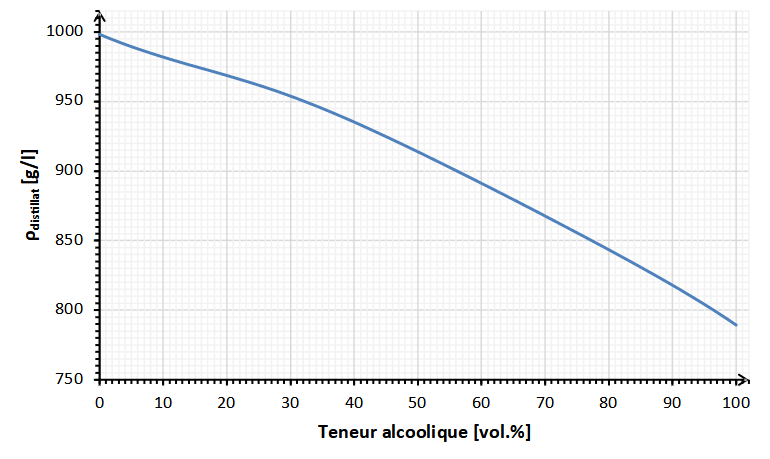
\includegraphics[scale=0.7]{vin3.png}
\end{document}